\documentclass{beamer}
\usetheme{Darmstadt}
\usecolortheme{default}
\usepackage{presentation}
\usepackage{amsmath}
\usepackage{mleftright}
\mleftright
\newcommand{\lcc}{T_{\ell}}
\newcommand{\mcc}{T_c}
\newcommand{\bigO}[1]{\mathcal{O}\left(#1\right)}
\newcommand{\bigOm}[1]{\Omega\left(#1\right)}
\newcommand{\softO}[1]{\tilde{\mathcal{O}}\left(#1\right)}
\newcommand{\softOm}[1]{\tilde{\Omega}\left(#1\right)}
\newcommand{\set}[1]{\left\{#1\right\}}
\newcommand{\card}[1]{\left\lvert#1\right\rvert}
\usepackage{booktabs}
\usepackage{xfrac}
\renewcommand{\sfrac}[2]{#1 / #2}
\UseCollection{xfrac}{plainmath}
\usepackage{algpseudocodex}
\usepackage{tikz, pgfplots}
\pgfplotsset{compat=newest}
\usetikzlibrary{shapes, shapes.misc, decorations, fit, backgrounds, positioning, patterns, shadows, calc, arrows, arrows.meta, trees}

\usetikzlibrary{external}
\tikzexternalize[prefix=tikzimages/]
\tikzset{>={Latex[width=2mm,length=2mm]}}
\newcommand\DoubleLine[7][4pt]{%
    \path(#2)--(#3)coordinate[at start](h1)coordinate[at end](h2);
    \draw[#4]($(h1)!#1!90:(h2)$)-- node [auto=left] {#5} ($(h2)!#1!-90:(h1)$); 
    \draw[#6]($(h1)!#1!-90:(h2)$)-- node [auto=right] {#7} ($(h2)!#1!90:(h1)$);
}
\tikzset{arrowhead/.style=
         {sloped,isosceles triangle,anchor=apex,fill=black,inner sep=2pt}}
\tikzset{
  point/.style={
    draw,
    circle,
    inner sep=0pt,
    outer sep=0pt,
    minimum size=0.1cm,
    fill
  }
}

\pgfdeclaredecoration{simple line}{initial}{
  \state{initial}[width=\pgfdecoratedpathlength-1sp]{\pgfmoveto{\pgfpointorigin}}
  \state{final}{\pgflineto{\pgfpointorigin}}
}
\tikzset{
   shift left/.style={decorate,decoration={simple line,raise=#1}},
   shift right/.style={decorate,decoration={simple line,raise=-1*#1}},
}

\title{Distributed Algorithms for Connectivity and MST in Large Graphs with Efficient Local Computation}
\author{Eric Ajieren, \alert{Khalid Hourani}, William K. Moses Jr., Gopal Pandurangan}
\date{January 4, 2022}
\institute{University of Houston}

\AtBeginSection[]
{
  \begin{frame}
    \frametitle{Table of Contents}
    \tableofcontents[currentsection]
  \end{frame}
}

\begin{document}

\frame{\titlepage}

\begin{frame}
    \frametitle{Table of Contents}
    \tableofcontents
\end{frame}

\section{Introduction}
\begin{frame}{The $k$-Machine Model}
    \begin{itemize}
        \item study distributed algorithms for large-scale graphs
        \item focus on connectivity and MST
        \item in $k$-machine model
              \begin{itemize}
                  \item $k \geq 2$ machines jointly perform computations on input graph
                  \item input graph distributed uniformly at random to $k$ machines
                        \begin{itemize}
                            \item $n$ nodes, $m$ edges
                            \item when a node is given to a machine, its \alert{adjacency list} is also
                            \item commonly called \alert{vertex centric} model
                        \end{itemize}
                  \item assume $n \gg k$ (e.g. $k = \bigO{n^{\varepsilon}}$)
              \end{itemize}
        \item typically, \alert{only consider communication cost}
              \begin{itemize}
                  \item message complexity --- number of communication rounds
              \end{itemize}
        \item traditionally done because network communication is much slower
              than local computation
              \begin{itemize}
                  \item less true as network speeds increase
              \end{itemize}
    \end{itemize}
\end{frame}

\begin{frame}{Our Results}
    \begin{itemize}
        \item we posit a new complexity measure
              \begin{itemize}
                  \item \alert{local computation cost} --- $\lcc$
                  \item measures the worst-case local computation cost among $k$ machines
              \end{itemize}
        \item refer to traditional communication complexity by $\mcc$
        \item lower bounds
              \begin{align*}
                  \lcc & = \bigOm{\frac{m + n}{k} + \Delta + k} \\
                  \mcc & = \bigOm{\frac{n}{k^2}}
              \end{align*}
        \item in practical implementations of $k$-machine model algorithms,
              often see suboptimal speedup
              \begin{itemize}
                  \item e.g. PageRank with $T_c = \bigO{\sfrac{n}{k}}$ but whose wall-clock
                        time is approximately $\sfrac{n}{k^{0.8}}$
              \end{itemize}
    \end{itemize}
\end{frame}

\begin{frame}
    \begin{itemize}
        \item analyze several algorithms under the new complexity measure
              \begin{tabular}{@{}lll@{}}\toprule
                  Algorithm                  & Round complexity          & Local runtime                        \\\midrule
                  Flooding                   & $\softO{\frac{n}{k} + D}$ & $\softO{\frac{m}{k} + \Delta + k}$   \\
                  Filtering                  & $\softO{\frac{n}{k}}$     & $\softO{\frac{m}{k} + n}$            \\
                  Improved Local Bor\r{u}vka & $\softO{\frac{n}{k}}$     & $\softO{\frac{m+n}{k} + \Delta + k}$ \\
                  Randomized CC              & $\softO{\frac{n}{k^2}}$   & $\softO{\frac{m+n}{k} + \Delta + k}$
              \end{tabular}
        \item many distributed algorithms that are optimal are often only optimal under \alert{communication complexity}
        \item as a byproduct of our analysis, we have two general results
              \begin{itemize}
                  \item the Node Distribution Lemma
                  \item the Mapping Lemma
              \end{itemize}
    \end{itemize}
\end{frame}

\begin{frame}
    \begin{lemma}[Node Distribution Lemma]
        Consider a graph $G$ of nodes $v_1, v_2, \hdots, v_n$ with associated
        non-negative real-valued ``weights'' $w(v)$ for each node $v$. Given a
        uniform, random distribution of the $n$ nodes to $k$ machines, as in the
        $k$-machine model, then, with probability at least $1 - \sfrac{1}{n^a}$ for any
        $a > 0$, the total weight of nodes at every machine is bounded above by
        \[\bigO{T_{\text{avg}}+\log{n}\cdot w_{\text{max}}}\]
        where $T_{\text{avg}}=\frac{1}{k}\sum_{i=1}^n w(v_i)$ and
        $w_{\text{max}} = \text{max}\set{w(v_i)}$.
    \end{lemma}
\end{frame}

\begin{frame}
    \begin{lemma}[Mapping Lemma]\label{lem:more-acc-mapping-lemma}
        Let an \(n\)-node, \(m\)-edge graph \(G\) be partitioned among the \(k\)
        machines as \(N = \set{p_1, \ldots, p_k}\). Then with probability at
        least \(1 - \sfrac{1}{n^\alpha}\), where \(\alpha > 1\) is an arbitrary
        fixed constant, the following bounds hold:
        \begin{enumerate}
            \item The number of vertices mapped to any machine is \(\bigO{n/k}\).
            \item The number of edges mapped to any machine is \(\mathcal{O}(m/k + \Delta \log n)\).
            \item The number of edges mapped to any link of the network is \(\bigO{m/k^2 + n/k}\).
        \end{enumerate}
    \end{lemma}
\end{frame}
\section{Parallel Flooding}
\begin{frame}
    \begin{itemize}
        \item the algorithm can be described from the perspective of a node
              \begin{itemize}
                  \item each node chooses an ID uniformly at random in $[1, n^4]$
                  \item each node floods its ID
                  \item upon receiving a message (with an ID), if the new ID is
                        greater than the current ID, the node updates its ID and
                        floods
              \end{itemize}
    \end{itemize}
\end{frame}


\begin{frame}
    \onslide<1-10>{
        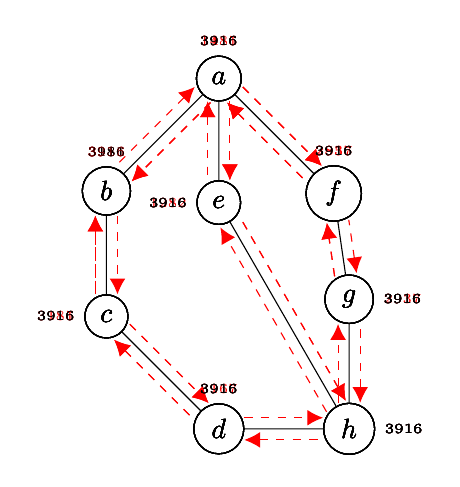
\begin{tikzpicture}
            \onslide<1>{
                \node[draw,circle] (a) {$a$};
                \node[draw,circle,below left=of a]  (b)  {$b$};
                \node[draw,circle,below=of a] (e) {$e$};
                \node[draw,circle,below right=of a] (f) {$f$};
                \node[draw,circle,below=of b] (c) {$c$};
                \node[draw,circle,below right=of c] (d) {$d$};
                \node[draw,circle,right=of d] (h) {$h$};
                \node[draw,circle,above=of h] (g) {$g$};
            }

            \onslide<2-3>{
            \node[draw,label=above:{\tiny\textcolor{red}{1415}},circle] (a) {$a$};
            \node[draw,label=above:{\tiny\textcolor{red}{3181}},circle,below left=of a]  (b)  {$b$};
            \node[draw,label=left:{\tiny\textcolor{red}{1282}},circle,below=of a] (e) {$e$};
            \node[draw,label=above:{\tiny\textcolor{red}{2855}},circle,below right=of a] (f) {$f$};
            \node[draw,label=left:{\tiny\textcolor{red}{5}},circle,below=of b] (c) {$c$};
            \node[draw,label=above:{\tiny\textcolor{red}{3167}},circle,below right=of c] (d) {$d$};
            \node[draw,label=right:{\tiny\textcolor{red}{3916}},circle,right=of d] (h) {$h$};
            \node[draw,label=right:{\tiny\textcolor{red}{2937}},circle,above=of h] (g) {$g$};
            }

            \draw (a) -- (b) -- (c) -- (d) -- (h) -- (g) -- (f) -- (a);
            \draw (a) -- (e) -- (h);

            \onslide<3>{
                \DoubleLine{a}{f}{->,red,dashed}{}{<-,red,dashed}{}
                \DoubleLine{a}{e}{->,red,dashed}{}{<-,red,dashed}{}
                \DoubleLine{a}{b}{->,red,dashed}{}{<-,red,dashed}{}
                \DoubleLine{b}{c}{->,red,dashed}{}{<-,red,dashed}{}
                \DoubleLine{c}{d}{->,red,dashed}{}{<-,red,dashed}{}
                \DoubleLine{d}{h}{->,red,dashed}{}{<-,red,dashed}{}
                \DoubleLine{h}{g}{->,red,dashed}{}{<-,red,dashed}{}
                \DoubleLine{h}{e}{->,red,dashed}{}{<-,red,dashed}{}
                \DoubleLine{g}{f}{->,red,dashed}{}{<-,red,dashed}{}
            }

            \onslide<4-5>{
            \node[draw,label=above:{\tiny\textcolor{red}{3181}},circle] (a) {$a$};
            \node[draw,label=above:{\tiny3181},circle,below left=of a]  (b)  {$b$};
            \node[draw,label=left:{\tiny\textcolor{red}{3916}},circle,below=of a] (e) {$e$};
            \node[draw,label=above:{\tiny\textcolor{red}{2937}},circle,below right=of a] (f) {$f$};
            \node[draw,label=left:{\tiny\textcolor{red}{3181}},circle,below=of b] (c) {$c$};
            \node[draw,label=above:{\tiny\textcolor{red}{3916}},circle,below right=of c] (d) {$d$};
            \node[draw,label=right:{\tiny3916},circle,right=of d] (h) {$h$};
            \node[draw,label=right:{\tiny\textcolor{red}{3916}},circle,above=of h] (g) {$g$};
            }

            \onslide<5>{
                \DoubleLine{a}{f}{->,red,dashed}{}{<-,red,dashed}{}
                \DoubleLine{a}{e}{->,red,dashed}{}{<-,red,dashed}{}
                \DoubleLine{c}{d}{->,red,dashed}{}{<-,red,dashed}{}
                \DoubleLine{g}{f}{->,red,dashed}{}{draw=none}{}
                \DoubleLine{h}{e}{draw=none}{}{<-,red,dashed}{}
            }

            \onslide<6-7>{
            \node[draw,label=above:{\tiny\textcolor{red}{3916}},circle] (a) {$a$};
            \node[draw,label=above:{\tiny3181},circle,below left=of a]  (b)  {$b$};
            \node[draw,label=left:{\tiny3916},circle,below=of a] (e) {$e$};
            \node[draw,label=above:{\tiny\textcolor{red}{3916}},circle,below right=of a] (f) {$f$};
            \node[draw,label=left:{\tiny\textcolor{red}{3916}},circle,below=of b] (c) {$c$};
            \node[draw,label=above:{\tiny3916},circle,below right=of c] (d) {$d$};
            \node[draw,label=right:{\tiny3916},circle,right=of d] (h) {$h$};
            \node[draw,label=right:{\tiny3916},circle,above=of h] (g) {$g$};
            }

            \onslide<7>{
                \DoubleLine{a}{f}{->,red,dashed}{}{<-,red,dashed}{}
                \DoubleLine{a}{b}{->,red,dashed}{}{draw=none}{}
                \DoubleLine{c}{b}{->,red,dashed}{}{draw=none}{}
            }

            \onslide<8> {
            \node[draw,label=above:{\tiny3916},circle] (a) {$a$};
            \node[draw,label=above:{\tiny\textcolor{red}{3916}},circle,below left=of a]  (b)  {$b$};
            \node[draw,label=left: {\tiny3916},circle,below=of a] (e) {$e$};
            \node[draw,label=above:{\tiny3916},circle,below right=of a] (f) {$f$};
            \node[draw,label=left: {\tiny3916},circle,below=of b] (c) {$c$};
            \node[draw,label=above:{\tiny3916},circle,below right=of c] (d) {$d$};
            \node[draw,label=right:{\tiny3916},circle,right=of d] (h) {$h$};
            \node[draw,label=right:{\tiny3916},circle,above=of h] (g) {$g$};
            }
            \onslide<9> {
            \node[draw,label=above:{\tiny3916},circle] (a) {$a$};
            \node[draw,label=above:{\tiny\textcolor{red}{3916}},circle,below left=of a]  (b)  {$b$};
            \node[draw,label=left: {\tiny3916},circle,below=of a] (e) {$e$};
            \node[draw,label=above:{\tiny3916},circle,below right=of a] (f) {$f$};
            \node[draw,label=left: {\tiny3916},circle,below=of b] (c) {$c$};
            \node[draw,label=above:{\tiny3916},circle,below right=of c] (d) {$d$};
            \node[draw,label=right:{\tiny3916},circle,right=of d] (h) {$h$};
            \node[draw,label=right:{\tiny3916},circle,above=of h] (g) {$g$};
            }

            \onslide<10> {
            \node[draw,label=above:{\tiny3916},circle] (a) {$a$};
            \node[draw,label=above:{\tiny3916},circle,below left=of a]  (b)  {$b$};
            \node[draw,label=left: {\tiny3916},circle,below=of a] (e) {$e$};
            \node[draw,label=above:{\tiny3916},circle,below right=of a] (f) {$f$};
            \node[draw,label=left: {\tiny3916},circle,below=of b] (c) {$c$};
            \node[draw,label=above:{\tiny3916},circle,below right=of c] (d) {$d$};
            \node[draw,label=right:{\tiny3916},circle,right=of d] (h) {$h$};
            \node[draw,label=right:{\tiny3916},circle,above=of h] (g) {$g$};
            }
        \end{tikzpicture}
    }
\end{frame}

\begin{frame}
    \begin{itemize}
        \item in order to simulate this in the $k$-Machine Model, each machine $M$
              \begin{itemize}
                  \item maintains list of nodes on the machine in descending-order of ID
                  \item iterate through list and simulate each node individually
                        \begin{itemize}
                            \item when $u$ located on $M$ sends a message to $v$ on $M'$, $M$ sends the appropriate message to $M'$
                        \end{itemize}
                  \item after some $\bigO{\sfrac{n\log{n}}{k} + D}$ rounds,
                        aggregate all IDs located on machine $M$ and send them to
                        machine $M_1$
              \end{itemize}
        \item Finally, machine $M_1$ counts the number of distinct IDs (which is the number of connected components) and broadcasts it to all machines
    \end{itemize}
\end{frame}

\begin{frame}
    \begin{theorem}\label{thm:flooding-thm}
        With high probability, the above algorithm correctly counts the number
        of connected components with
        \begin{align*}
            \lcc & = \bigO{(m/k + \Delta\log n) \log n + k} \\
            \mcc & = \bigO{n\log n/k + D}
        \end{align*}
    \end{theorem}
    \begin{proof}
        \begin{itemize}
            \item with Chernoff Bounds, can show that a node $v$ will update max-ID
                  $\bigO{\log{n}}$ times with probability $1 - \sfrac{1}{n^a}$
            \item $v$ will receive $\bigO{\deg(v)\log{n}}$ higher IDs
            \item when max-ID is updated, $v$ sends to $\deg(v)$ nodes, totaling $\bigO{\deg(v)\log{n}}$
            \item maximum runtime is therefore $\bigO{\Delta\log{n}}$.
        \end{itemize}
    \end{proof}
\end{frame}

\begin{frame}
    \begin{proof}
        \begin{itemize}
            \item apply node distribution lemma on the degree of nodes
                  \begin{align*}
                      \lcc & = \bigO{\frac{1}{k}\left(\sum_{i=1}^n (d(v_i) \log n)\right) + \log n \cdot \Delta \log n} \\
                           & = \bigO{\left(\frac{m}{k} + \Delta \log n\right) \log n}
                  \end{align*}
            \item in the worst case, a machine sends/receives messages from all other machines, totaling
                  \[\bigO{\left(\frac{m}{k} + \Delta \log n\right) \log n + k}\]
        \end{itemize}
    \end{proof}
\end{frame}

\begin{frame}
    \begin{lemma}
        The communication complexity of the algorithm is $\bigO{n\log n/k + D}$
        with high probability.
    \end{lemma}
    \begin{proof}
        \begin{itemize}
            \item by conversion theorem (see~), total number of broadcasts is $\bigO{\sfrac{B\log{n}}{(kW)} + D}$ where $W$ is the bandwidth
            \item taking $W = \bigO{\log{n}}$
            \item by mapping lemma, $\bigO{\log{n}}$ broadcasts for a particular
                  node with probability $1 - \sfrac{1}{n^2}$
            \item by union bound, $\bigO{\log{n}}$ broadcasts for all nodes with
                  probability $1 - \sfrac{1}{n}$
            \item thus, $\bigO{n\log{n}}$ broadcasts initiated with high probability
        \end{itemize}
    \end{proof}
\end{frame}
\section{Filtering-Based MST}
\begin{frame}{Preliminaries}
    \begin{itemize}
        \item uses three procedures:
        \item Kruskal's algorithm --- outputs an MST in $\bigO{m\log{m}}$ rounds
        \item maximal matching a clique of size $n$
              \begin{itemize}
                  \item done by simply sorting IDs and matching node $2i - 1$ to node $2i$
              \end{itemize}
        \item distributed routing in a clique
              \begin{itemize}
                  \item node $u$ wants to send $f$ messages to a different node $v$
                  \item phase 1:
                        \begin{itemize}
                            \item divide messages into groups of $\sfrac{f}{(n-1)}$
                            \item append destination id to messages
                            \item send one group per edge
                        \end{itemize}
                  \item phase 2:
                        \begin{itemize}
                            \item each node forwards its message to the destination
                        \end{itemize}
              \end{itemize}
    \end{itemize}
\end{frame}
\begin{frame}{The Algorithm}
    \begin{itemize}
        \item each machine $M$ maintains
              \begin{itemize}
                  \item a graph $G_M$
                        \begin{itemize}
                            \item initially comprised of subgraph induced by edges in $M$
                        \end{itemize}
                  \item ordered list $H_M$ comprised of IDs of all machines
              \end{itemize}
        \item each machine $M$ executes at most $2\log{k}$ phases of:
              \begin{itemize}
                  \item if $M$ received information about new edges in previous phase,
                        it updates $G_M$ accordingly, then runs Kruskal's to remove cycles
                  \item if $\card{H_M} = 1$, terminate. Use matching procedure on $H_M$ to
                        match with machine $M'$. If the ID of $M$ is greater than that of $M'$,
                        use routing procedure to send $G_M$ to $M'$
                  \item For any machine $M''$ in $H_M$, if $M''$ matched with a machine with
                        a lower ID than $M''$, remove $M''$ from $H_M$. If $M$ is such a machine,
                        terminate
              \end{itemize}
        \item at the end of the algorithm, the machine with the lowest ID will have
              the entire MST
    \end{itemize}
\end{frame}

\begin{frame}
    \begin{itemize}
        \item Correctness is fairly straightforward
        \begin{itemize}
            \item if $e$ is a cut edge, then it will never be removed by Kruskal's
            \item the matching algorithm guarantees that after $2\log{k}$ phases, the lowest
            ID machine will contain $e$
        \end{itemize}
    \end{itemize}
\end{frame}
\section{Determinstic Bor\o{u}vka-Style Algorithm}
\begin{frame}
    \begin{itemize}
        \item we present two deterministic algorithms
        \item however, a quick review of Bor\o{u}vka's
        \item each machine stores a disjoint-set (union-find) $\mathcal{M}$
        \item in each phase:
              \begin{itemize}
                  \item an MOE is found for each fragment
                  \item fragments are merged along MOEs
              \end{itemize}
    \end{itemize}
\end{frame}

\begin{frame}{Algorithm 1}
    \begin{itemize}
        \item each phase consists of two steps
              \begin{itemize}
                  \item for any node $v$ in $M$, $M$ iterates through the adjacency
                        list of $v$ and performs \textproc{Find} until it finds an edge belonging
                        to another fragment, after which it broadcasts this MOE
                  \item $M$ merges fragments: if $(u, v)$ is an MOE, $M$ updates $\mathcal{M}$ with $\Call{Union}{u, v}$.
              \end{itemize}
    \end{itemize}
\end{frame}

\begin{frame}{Algorithm 2 --- The Improved Algorithm}
    \begin{itemize}
        \item can improve $\lcc$
        \item rather than broadcasting MOEs, simulate unicast version (as in GHS)
        \item additionally, we filter to reduce the number of edges in each machine to $\bigO{n}$
              \begin{itemize}
                  \item machines create MSFs of their local subgraphs using Kruskal's
                  \item ``discard'' edges that are not part of local MSF
                  \item the remaining (at most $k(n-1)$ edges whp) are the only MST edges reamining
              \end{itemize}
        \item algorithm then continues on remaining subgraphs
    \end{itemize}
\end{frame}

\begin{frame}
    \begin{itemize}
        \item for a fixed machine $M$ and fragment $f$
        \item set $\texttt{LOE} = \infty$
              \begin{itemize}
                  \item iterate through edges in $f$ --- for edge $(u, v)$ with $u$ in $M$, send a message to the machine containing $v$ with IDs of $u$ and $v$ and fragment ID of $f$
                  \item for each message $(u, v, f)$, if the fragment ID of $v$ is different than the received fragment ID, respond with original fragment ID and fragment ID of $f$
                  \item update $\texttt{LOE} = \Call{min}{\texttt{LOE}, w}$ for each message received corresponding to $f$, where $w$ is the weight
                        of the outgoing edge
                \item broadcast the \texttt{LOE} and fragment ID
              \end{itemize}
        \item from the broadcast of the \texttt{LOE}s, each machine locally determines the global MOE for any fragment it contains
        \item the machine then merges fragments
    \end{itemize}
\end{frame}

\begin{frame}{Merging}
    \begin{itemize}
        \item Note that we cannot merge all fragments at once, as that takes time proportial to the length of the fragment chain
        \item use a technique similar to \alert{controlled GHS}
        \begin{itemize}
            \item create rooted tree $F$ --- each node is a fragment and there is an edge between nodes if they share an MOE
            \item construct maximal matching (using e.g. Cole-Vishkin)
            \item merge all matches edges and any edge where \alert{exactly} one
            endpoint is matched
        \end{itemize}
    \end{itemize}
\end{frame}
\section{An Almost-Optimal Randomized Algorithm}
\begin{frame}{Sketch-Based Randomized Algorithm}
    \begin{itemize}
        \item we analyze the 2018 SPAA algorithm of Pandurangan, Robinson, and Scquizzato
        \item optimal up to polylog factors in terms of round complexity
        \begin{itemize}
            \item but $\softO{n^2}$ local computation complexity
        \end{itemize}
        \item the algorithm is similar to Bor\r{u}vka's algorithm, with
              the output being a \alert{labeling} of the nodes, such that nodes in the same component have the same label
        % \item component also have a \alert{component proxy} that handles finding MOEs and merging for the component
        % \item initially, each node has label equal to its ID (forming its own component) and is its own component proxy
        % \item to load balance communication and computation, component proxies are chosen randomly among the machines
        % \item given a component $f$ and a machine $M$, the set of nodes belonging
        %       to $f$ in $M$ are called the \alert{component part}
        \item relies on \alert{linear graph sketches} to efficiently merge multiple components
    \end{itemize}
\end{frame}

\begin{frame}{Sketches}
    \begin{itemize}
        \item sketches are found by forming a vector of length
              $\binom{n}{2}$ for each node $v$ and and appropriate choice of an
              $\bigO{\log^2{n}} \times \binom{n}{2}$ matrix. This requires $\softOm{n^2}$ local computation time.
        \item can be improved by using the 2015 sketches of King, Kutten, and Thorup
        \item instead of storing vectors of length $\binom{n}{2}$, a leader machine broadcasts an \alert{odd hash function}
        \item each component uses this hash function to find an MOE
        \item brings it to $\lcc = \softO{\sfrac{(m+n)}{k} + \Delta + k}$
        \begin{itemize}
            \item optimal, up to polylog factors!
        \end{itemize}
    \end{itemize}
\end{frame}

% \begin{frame}
%     \begin{itemize}
%         \item each component uses this hash function to find an MOE as follows
%               \begin{itemize}
%                   \item each node in a component part evaluates $\sum_{\text{incident edges } e} h(e)
%                             \bmod{2}$
%                   \item this sum is aggregated among the nodes in a component part by the
%                         corresponding machine
%                   \item the sums of each part of the component are aggregated to the
%                         corresponding component proxy machine.
%                   \item If the sum is 1, we conclude with some constant probability
%                         $\varepsilon$ that an outgoing edge exists out of the component
%                         \begin{itemize}
%                             \item By restricting the edges considered to be those within some range $[i, j]$, can (like binary search) determine an MOE with constant probability
%                             \item repeating this process $\bigOm{\log{n}}$ times yields an
%                                   MOE whp for a single component
%                             \item by union bound, we have MOE for all components whp
%                         \end{itemize}
%               \end{itemize}
%     \end{itemize}
% \end{frame}
\end{document}
